\documentclass[fleqn,11pt]{article}

\usepackage{datetime}
\newcommand{\ver}{version 0.10\xspace}
\newdateformat{mydate}{\THEDAY~\monthname[\THEMONTH]~\THEYEAR}
\newcommand{\auth}{Fernando D. Bianchi}
\newcommand{\email}{febianchi@itba.edu.ar}
\newcommand{\web}{http://fdbianchi.github.io}

\usepackage{graphicx,epstopdf}
\usepackage{wrapfig}
%
% margenes
\usepackage[a4paper,left=2.5cm,right=2.5cm,top=2.5cm,bottom=2.5cm]{geometry}
\setlength{\parskip}{2ex}

% fonts
\usepackage{bera}
\usepackage[T1]{fontenc}
%
% for link and cross-references
\usepackage{color}
\definecolor{clink}{rgb}{0,0,0.4}
\definecolor{ccite}{rgb}{0,0,0.4}
\usepackage[english]{hyperref}   % hipervículos
\hypersetup{colorlinks, backref, pdfpagemode=None, linkcolor=clink,
            citecolor=ccite, urlcolor=clink, pdfhighlight=/I, pdfstartview=FitH,
            pdfauthor=F.D.Bianchi, breaklinks}
\usepackage{url}
\newcommand{\weblink}[1]{\url{#1}}
%
% titles
\usepackage[nobottomtitles*]{titlesec}
\definecolor{MyDarkBlue}{rgb}{0,0.08,0.45}
\titleformat{\chapter}
    {\sffamily\bfseries\LARGE}{}{0ex}{}
\titlespacing*{\chapter}%
    {-0.5cm}{7.5ex plus 0.2ex minus 0.2ex}{3.5ex plus 0.2ex minus 0.2ex}%
\titleformat{\section}%
    {\sffamily\bfseries\Large%
     }{\thesection}{1.0em}{}[{\color{MyDarkBlue}{\titlerule[0.7pt]}}]%
\titlespacing*{\section}%
    {-0.5cm}{6.5ex plus 0.2ex minus 0.2ex}{3.0ex plus 0.2ex minus 0.2ex}%
\titleformat{\subsection}%
    {\sffamily\bfseries\large}{\thesubsection}{0.8em}{}[]%
\titlespacing*{\subsection}%
    {-0.5cm}{4.5ex plus 0.2ex minus 0.2ex}{2.0ex plus 0.2ex minus 0.2ex}%
\titleformat{\subsubsection}%
    {\sffamily\bfseries\normalsize}{}{0.0em}{}%[\titlerule]%
\titlespacing*{\subsubsection}%
    {0cm}{0.5ex plus 0.1ex minus 0.1ex}{0.1ex plus 0.1ex minus 0.1ex}%
\renewcommand{\abstractname}{\vspace{-\baselineskip}}
% headers
\usepackage{fancyhdr}
\fancypagestyle{headings}{%
    \fancyhf{} % clear all six fields
    \fancyfoot[L]{\small\textcolor{gray}{\awtool, \ver~-~\mydate\today}}
    \fancyfoot[R]{\small\textcolor{gray}{\thepage}}
    \renewcommand{\headrulewidth}{0pt}
    \let\FootRule\footrule
    \renewcommand\footrule{\color{gray}\FootRule}    \renewcommand{\footrulewidth}{1pt}}
\pagestyle{headings}
% new environments
\usepackage{enumitem}
\setlist[itemize]{label=-,topsep=0ex,parsep=0ex,partopsep=0ex,%
        leftmargin=3ex,itemsep=1.2ex}
% tables
\usepackage{booktabs,array}
% for matlab code
\usepackage{listings}
\usepackage{matlab-prettifier}
\lstdefinestyle{mystyle}{
    style=Matlab-editor,
    basicstyle=\mlttfamily,
    backgroundcolor=\color{gray!15},
    rulecolor=\color{gray!15},
    frame=single,
    xleftmargin=2mm,
    framexleftmargin=1mm,
    framextopmargin=0mm,
    framexbottommargin=0mm,
    aboveskip={1.5ex},
    belowskip={0.0ex}
}
\definecolor{ccode}{rgb}{0,0.08,0.45}
\lstMakeShortInline[style=mystyle,basicstyle=\mlttfamily\color{ccode}]!
\lstnewenvironment{code}{\lstset{style=mystyle}}{}
\newcommand{\lcode}[1]{\textbf{%
    \lstinline[style=mystyle]{#1}}}


% some symbols definition
\usepackage{amssymb,amsmath}
\usepackage{mathrsfs,bm}

\newcommand{\MT}{MatLab}
% Mathematic symbols
\newcommand{\Linf}{\mathcal{L}_\infty}
\newcommand{\Hinf}{\mathcal{H}_\infty}
\newcommand{\ltwo}{\mathcal{L}_2}
\newcommand{\Htwo}{\mathcal{H}_2}
\newcommand{\Nset}{\mathbb{N}}
\newcommand{\Rset}{\mathbb{R}}
\newcommand{\Cset}{\mathbb{C}}
\newcommand{\jw}{\jmath\omega}

% Operators
\newcommand{\diag}{\mathrm{diag}}
\newcommand{\gr}{^\circ}
\newcommand{\co}{\mathrm{co}}
\newcommand{\eqdef}{\buildrel \triangle \over =}
\newcommand{\ninf}[1]{\left\|#1\right\|_{\infty}}
\newcommand{\nugap}{$\nu$-gap\xspace}
\newcommand{\lftu}[2]{\mathcal{F}_u\left(#1,#2\right)}
\newcommand{\lftl}[2]{\mathcal{F}_l\left(#1,#2\right)}

% environments
\newtheorem{teo}{Theorem}[section]
\newtheorem{coro}{Corollary}[section]
\newtheorem{defin}{Definition}[section]
\newtheorem{lema}{Lemma}[section]
\newtheorem{example}{Example}[section]
\newcommand{\proof}{\paragraph*{Proof}}
\newcommand{\qed}{\hfill$\Box$}

\newcommand{\nom}{\mathrm{nom}}
\newcommand{\rf}{\mathrm{ref}}
\usepackage{bbm}
\newcommand{\oneM}{\mathbbm{1}}
\newcommand{\slfrac}[2]{\left.#1\middle/#2\right.}
\newcommand{\real}{\mathfrak{Re}}
\newcommand{\kp}{\beta}
\newcommand{\ki}{\alpha}
\newcommand{\der}[1]{\frac{d#1}{dt}}

% Texts
\usepackage{xspace}
\newcommand{\apr}{{\em a priori}\ }
\newcommand{\apo}{{\em posteriori}\ }
\newcommand{\ie}{{\em i.e.}\xspace}
\newcommand{\eg}{{\em e.g.}\xspace}
\newcommand{\etal}{{\em et al.}\xspace}

% variables and matrices
\newcommand{\p}{\rho}
\newcommand{\Pset}{\mathcal{P}}
\newcommand{\Pdset}{\mathcal{P}_d}
\newcommand{\Xu}{\mathbf{X}}
\newcommand{\Yu}{\mathbf{Y}}
\newcommand{\Pu}{\mathbf{P}}
\newcommand{\Su}{\mathbf{S}}
\newcommand{\Tu}{\mathbf{T}}
\newcommand{\Gu}{\mathbf{G}}
\newcommand{\Lu}{\mathbf{L}}
\newcommand{\Hu}{\mathbf{H}}
\newcommand{\Qu}{\mathbf{Q}}
\newcommand{\Zu}{\mathbf{Z}}
\newcommand{\Uu}{\mathbf{U}}
\newcommand{\Vu}{\mathbf{V}}
\newcommand{\Au}{\mathbf{\hat A}}
\newcommand{\Bu}{\mathbf{\hat B}}
\newcommand{\Cu}{\mathbf{\hat C}}
\newcommand{\Du}{\mathbf{\hat D}}
\newcommand{\aw}{\mathrm{aw}}
\newcommand{\Aw}{A_{\aw}}
\newcommand{\Bw}{B_{\aw}}
\newcommand{\Cwu}{C_{\aw,u}}
\newcommand{\Cwy}{C_{\aw,y}}
\newcommand{\Dwu}{D_{\aw,u}}
\newcommand{\Dwy}{D_{\aw,y}}
\newcommand{\sat}{\mathrm{sat}}
\newcommand{\Dz}{\mathrm{Dz}}
\newcommand{\awtool}{\textbf{AWtools}\xspace}
\newcommand{\lpvtool}{\textbf{LPVtools}\xspace}

\usepackage{cleveref}
\crefname{figure}{Figure}{Figures}
\crefname{table}{Table}{Tables}
\crefname{section}{Section}{Sections}
\crefname{equation}{}{}
\crefrangeformat{equation}{(#3#1#4)-(#5#2#6)}
\usepackage[numbers]{natbib}


\begin{document}

\title{\awtool: a toolbox for designing MIMO anti-windup strategies}
\author{\auth\\\weblink{\web}~-~\email}
\date{\ver~-~\mydate\today}
%
\maketitle{}

\begin{abstract}
    \awtool is a short toolbox for Matlab aimed to design anti-windup (AW) strategies for MIMO plants. The design tools are based on the traditional two-step approaches, in which the AW compensator is designed after a controller is tuned without considering saturation. \awtool covers LTI and LPV plants and is based on the comprime factor formulation introduced in \cite{Turner2004,Skogestad2005}.
\end{abstract}

\section{Getting started}\label{sec:gt}

This toolbox provides the synthesis function
\begin{code}
[Kaw,Taw,g] = awsyn(G,K,method,nr,opts,F1,F2);
\end{code}
to design the anti-windup (AW) compensation scheme depicted in \cref{fig:AW1} \citep{Turner2004}, where !Kaw! is the combination of the controller !K! and the AW compensator !Taw!.

\begin{figure}
    \centering
    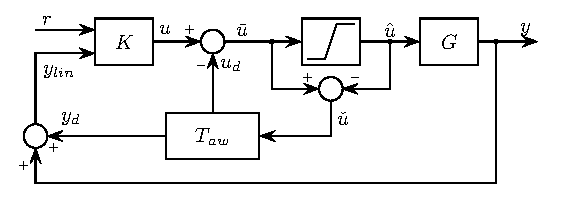
\includegraphics{figs/fig_sch_AWcomp_1}\\
    \caption{Anti-windup compensation scheme}\label{fig:AW1}
\end{figure}

The plant !G! and the controller !K! can be LTI or LPV systems. These systems can be modelled with Control System/Robust Control Toolbox objects, LMI Toolbox objects, or LPV objects from \lpvtool. The input argument !method! is a string defining the synthesis method:
\begin{itemize}
    \item !'fsec'!: produces a full order AW compensator !Taw! designed according to the method proposed in \citep{Skogestad2005} based on sector boundedness,
    \item !'fsgt'!: produces a full order AW compensator !Taw! designed using Small Gain Theorem arguments,
    \item !'ssec'!: produces a static AW compensator !Taw! designed according to the method proposed in \citep{Turner2004} based on sector boundedness,
    \item !'psec'!: produces a low-order AW compensator !Taw! using the same ideas as !'ssec'! but with the addition of two filters, !F1! and !F2!.
\end{itemize}

The argument !nr! is the size of the reference $r$ for cases of 2-dof controllers, by default it is assumed zero, \ie, the controller input is the error $e=r-y_{lin}$.

The argument !opts! is a struct with settings for the design algorithm. This will be explained next as it depends on the particular design method.

\section{Design methods}\label{sec:design}

Consider an LPV plant of the form
\begin{equation}\label{eq:Plant}
    G(\p):\left\{
        \begin{aligned}
            \dot x &= A(\p) x + B(\p)\hat{u},\\
                 y &= C(\p)x + D(\p)\hat{u},
        \end{aligned}
        \right.
\end{equation}
and the controller
\begin{equation}\label{eq:Ctrller}
    K(\p):\left\{
        \begin{aligned}
            \dot x_c &= A_c(\p) x + B_{cr}(\p) r + B_{cy}(\p) y_{lin},\\
                  u  &= C_c(\p) x + D_{cr}(\p) r + D_{cy}(\p) y_{lin},
        \end{aligned}
        \right.
\end{equation}
where $x\in\Rset^{n_s}$ is the plant state vector, $\hat{u}\in\Rset^{n_u}$ is the control input, $y\in\Rset^{n_y}$ is the controlled output, $x_c\in\Rset^{n_k}$ is the controller state vector, $u\in\Rset^{n_u}$ is the controller output, and $r\in\Rset^{n_r}$ is the reference. The parameter $\p$ takes values in a compact set $\Pset$. Notice that an LPV model evaluated at a constant parameter value reduces to an LTI model. Hence, the explanations will be focused on LPV models since the LTI ones can be considered as a particular case.

The AW compensation scheme in \cref{fig:AW1} consists of two compensation terms: one acting on the controller output $u_d\in\Rset^{n_u}$ and another on the controller input $y_d\in\Rset^{n_y}$. Defining
\begin{equation*}
    \begin{bmatrix} u_d \\ y_d \end{bmatrix} =
    T_{\aw}(\p)\check{u}
     = \begin{bmatrix} M(\p)-I \\ N(\p) \end{bmatrix}\check{u},
\end{equation*}
where $N=G M$ and $\check{u} = u - u_d - \sat(\bar{u}) = u - u_d - \hat{u}$. It can be proved, after some system manipulations, that the compensation scheme in \cref{fig:AW1} is equivalent to the scheme in \cref{fig:AW2}. After this reformulation and providing the nominal closed-loop system is stable, it is clear that the design of the AW compensator reduces to ensuring stability of the closed-loop system formed by $M-I$ and the dead-zone operator (nonlinear loop) and minimizing the effect of the $y_d$ on the controlled variable (disturbance filter).

\begin{figure}
    \centering
    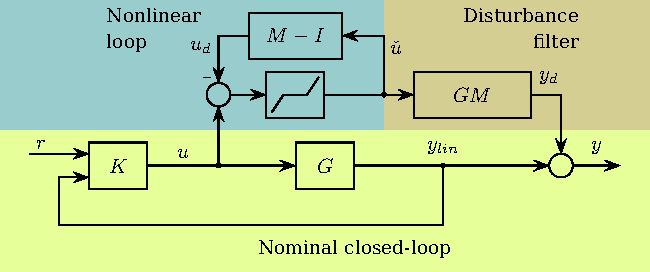
\includegraphics{figs/fig_sch_AWcomp_2}\\
    \caption{Equivalent representation of the anti-windup compensation scheme in \cref{fig:AW1}}\label{fig:AW2}
\end{figure}

The AW compensation schemes can be:
\begin{itemize}
    \item \emph{static}:
        \begin{equation*}
            T_{\aw}(\p):\left\{
                \begin{aligned}
                    u_d &= \Dwu(\p)\check{u},\\
                    y_d &= \Dwy(\p)\check{u},
                \end{aligned}
                \right.
        \end{equation*}
    \item \emph{low-order}:
        \begin{equation*}
            T_{\aw}(\p):\left\{
                \begin{aligned}
                    u_d &= F_1(s)\Dwu(\p)\check{u},\\
                    y_d &= F_2(s)\Dwy(\p)\check{u},
                \end{aligned}
                \right.
        \end{equation*}
    \item \emph{full order} (\ie with the same order than the plant $G$):
        \begin{equation*}
            T_{\aw}(\p):\left\{
                \begin{aligned}
                    \dot x_e &= \Aw(\p) x_e  + \Bw(\p)\check{u},\\
                         u_d &= \Cwu(\p) x_e + \Dwu(\p)\check{u},\\
                         y_d &= \Cwy(\p) x_e + \Dwy(\p)\check{u}.
                \end{aligned}
                \right.
        \end{equation*}
\end{itemize}
Therefore, the controller with the AW compensator results:
\begin{itemize}
    \item \emph{in the static case}
        \begin{equation*}
            K_{\aw}(\p):\left\{
                \begin{aligned}
                    \dot x_c &= A_c(\p) x_c + B_{cr}(\p)r + B_{cy}(\p)y + B_{cy}(\p)\Dwy(\p)\check{u},\\
                    \bar u &= C_c(\p) x_c + D_{cr}(\p)r + D_{cy}(\p)y  +(D_{cy}(\p)\Dwy(\p) - \Dwu(\p))\check{u},
                \end{aligned}
                \right.
        \end{equation*}
    \item \emph{in the low-order and full order cases}
        \begin{equation*}
            K_{\aw}(\p):\left\{
                \begin{aligned}
                    \dot x_c &= A_c(\p) x_c + B_{cy}(\p)\Cwy(\p) x_e + B_{cr}(\p)r + B_{cy}(\p)y + B_{cy}(\p)\Dwy\check{u},\\
                    \dot x_e &= \Aw(\p) x_e + \Bw(\p)\check{u},\\
                    \bar u &= C_c(\theta) x_c + (D_{cy}(\p)\Cwy(\p)-\Cwu(\p)) x_e + D_{cr}(\p)r + D_{cy}(\p)y  \\
                    &\hspace{6.5cm} +(D_{cy}(\p)\Dwy(\p)-\Dwu(\p))\check{u}.
                \end{aligned}
                \right.
        \end{equation*}
\end{itemize}

\section{Full order AW compensators}\label{sec:full}

In case the AW compensator is full order, \ie with the same order than the plant $G$, and if $M$ and $N$ are the coprime factors of the plant $G$ \citep{Xie2004}, the design of the AW compensator can be expressed as the design of a state-feedback gain fulfilling an induced $\mathcal{L}_2$ norm condition. More precisely, the design of the AW compensation consists in finding the matrix $H(\p)$ such that
\begin{equation}\label{eq:sysCL_f}
    \begin{bmatrix} M(\p)-I \\ N(\p) \end{bmatrix}:
    \left\{
        \begin{aligned}
            \dot{x}_e &= (A(\p)+B(\p)H(\p)) x_{e} + B(\p)\check{u}, \\
                     u_d &= H(\p) x_{e} ,\\
                     y_d &= (C(\p)+D(\p)H(\p)) x_{e} + D(\p)\check{u}.
        \end{aligned}\right.
\end{equation}
is internally stable and the operator $\check{u}\to y_d$ is small in a $\ltwo$ sense.

\subsection{Design based on sector boundedness (\lcode{method='fsec'})}\label{sec:fsec}

The dead-zone nonlinearity
\begin{equation*}
    \Dz(v_j) = v_j - \sat(v_j),
\end{equation*}
satisfies the inequality
\begin{equation*}
    \Dz(v_j)w_j(v_j-\Dz(v_j))\geq0,
\end{equation*}
for each input channel $j$ ($j=1,\dots,n_u$) and a positive weight $w_j$. Then, collecting the inequalities for all $j$, the nonlinearity satisfies
\begin{equation}\label{eq:full2-1}
    \Dz(v)^TW(v-\Dz(v))\geq0
\end{equation}
with $W=\diag(w_1,\dots,w_{n_u})>0$.

\citet{Skogestad2005} combine \cref{eq:full2-1} with the standard Bounded Real Lemma constraint to ensure internal stability and that the $\ltwo$-norm of the operator $\check{u}\to y_d$ is lower that $\gamma>0$. More concretely, substituting $v=u-u_d$ in \cref{eq:full2-1}, this inequality results
\begin{equation}\label{eq:full2-2}
    2\check{u}^TW(u-H(\p)x-\check{u})\geq0.
\end{equation}
The constraints on the $\ltwo$-norm of the operator $\check{u}\to y_d$ can be expressed as
\begin{equation}\label{eq:full2-3}
    \dot{V}(x)+y_d^Ty_d-\gamma^2\check{u}^T\check{u}<0,
\end{equation}
where the Lyapunov function is defined as $V(x)=x^T\Yu x$. Combining these inequalities using the S-procedure, the design of the AW compensator results in finding a positive definite matrix $\Yu>0$, a diagonal matrix $\Uu=\tau W^{-1}$ ($\tau>0$) and a general matrix function $\Lu(\p)$ such that
\begin{equation}\label{eq:lmi_FSEC}
    \begin{bmatrix}
    (A(\p)\Yu+B(\p)\Lu(\p))+(\star) & B(\p)\Uu-\Lu(\p) & 0 & (C(\p)\Yu+D(\p)\Lu(\p))^T\\
    \star & -2\Uu & I & \Uu D(\p)^T\\
    \star & \star & -\gamma I & 0\\
    \star & \star & \star & -\gamma I
    \end{bmatrix}<0,
\end{equation}
for all $\p\in\Pset$. Then, the state feedback gain $H$ is given by
\begin{equation*}
    H(\p)=\Lu(\p)\Yu^{-1}.
\end{equation*}


\subsection{Design based on Small Gain Theorem (\lcode{method='fsgt'})}\label{sec:fsgt}

The AW compensator \cref{eq:sysCL_f} can also be found using Small Gain Theorem concepts. In this line, the system \cref{eq:sysCL_f} is internally stable if the $\ltwo$-norm of the operator $\check{u}\to u_d$ is lower than $1$. Therefore, the design of the AW compensator can be stated as the following optimization problem:
\begin{align}
    \underset{H}{\text{minimize}}
       &\quad \gamma \label{eq:fsgt_1}\\
    \text{subtject to }&\quad ||GM||_{\ltwo}  < \gamma, \\
                       &\quad ||M-I||_{\ltwo} < 1 \label{eq:fsgt_3}.
\end{align}

Using the Bounded Real Lemma, the state feedback gain $H$ must satisfy the constraint
\begin{align}
    \begin{bmatrix}
    (A(\p)\Yu+B(\p)\Vu(\p))+(\star) & B(\p) & \Vu(\p)^T \\
    \star & -I & 0\\
    \star & \star & -I
    \end{bmatrix}&<0,\label{eq:lmi_FSGT_1}\\
    \begin{bmatrix}
    (A(\p)\Yu+B(\p)\Vu(\p))+(\star) & B(\p) & (C(\p)\Yu+D(\p)\Vu(\p))^T\\
    \star & -\gamma I & D(\p)^T\\
    \star & \star & -\gamma I
    \end{bmatrix}&<0,\label{eq:lmi_FSGT_2}
\end{align}
for all $\p\in\Pset$, with $\Yu>0$ and $H(\p)=\Vu(\p)\Yu^{-1}$.



\subsection{Computational aspects}\label{sec:fcomp}

Finding the state-feedback satisfying LMIs \cref{eq:lmi_FSEC,eq:lmi_FSGT_1,eq:lmi_FSGT_2} involves to solve an infinite dimensional optimization problem with infinity constraints. If the matrices $B$, $C$ and $D$ in the plant \cref{eq:Plant} are constants, the matrix $A$ is an affine function of $\p$ or polytopic, \ie,
\begin{equation*}
      A(\p) = \sum_{i=1}^{n_v}\alpha_i A_{i}
\end{equation*}
where
\begin{equation*}
    \p = \sum_{i=1}^{n_v}\alpha_i\p^i,\quad
    \alpha_1+\dots+\alpha_{n_v} = 1,\quad
    0\leq\alpha_i\leq1, \quad\forall\,i=1,\dots,n_v.
\end{equation*}
with $\p^i$ the vertices of the polytopic parameter set $\Pset$, and the matrix functions $\Lu$ and $\Vu$, respectively, are also affine or polytopic, LMIs \cref{eq:lmi_FSEC,eq:lmi_FSGT_1,eq:lmi_FSGT_2} are satisfied for all $\p\in\Pset$ if and only if they are satisfied at the vertices $\p^i$ of the polytope $\Pset$ \cite{Apkarian1995}.

When the previous conditions are not fulfilled, the feedback gains can be obtained by evaluating LMIs \cref{eq:lmi_FSEC,eq:lmi_FSGT_1,eq:lmi_FSGT_2} at a grid of points in the set $\Pset$. If the grid of points is sufficiently dense, it can be assumed that the computed feedback gains satisfy the constraints at the rest of points in $\Pset$ \cite{Apkarian1998,Wu1996}.

\awtool will analyze the plant matrices and will compute an polytopic $H$ when it is possible.

\section{Static and low-order AW compensators}\label{eq:stat}

In the case of a static AW compensator (\lcode{method='ssec'}),
\begin{equation}\label{eq:stat-1}
    \begin{bmatrix} u_d \\ y_d \end{bmatrix} =
    T_{aw}\check{u},
\end{equation}
it can be proved \citep{Turner2004} that
\begin{equation}\label{eq:stat-2}
    \begin{bmatrix} M(\p)-I \\ N(\p) \end{bmatrix} :
    \left\{
        \begin{aligned}
            \dot x_e &= \bar A(\p) x_e + (\bar{B}_0(\p) + \bar{B}_1(\p)T_{\aw}(\p)) \check{u},\\
               u_d &= \bar C_{u}(\p) x_e + (\bar{D}_{u,0}(\p) + \bar D_{u,1}(\p)T_{\aw}(\p)) \check{u},\\
               y_d &= \bar C_{y}(\p) x_e + (\bar{D}_{y,0}(\p) + \bar D_{y,1}(\p)T_{\aw}(\p)) \check{u},\\
        \end{aligned}
    \right.,
\end{equation}
where
\begin{align*}
    &\bar A(\p) = \begin{bmatrix}
                A(\p)+B(\p)\tilde\Delta(\p)D_{cy}(\p)C(\p) & B(\p)\tilde\Delta(\p) C_{c}(\p)\\
                B_{cy}(\p)\Delta(\p)C(\p) & A_{c}(\p)+B_{cy}(\p)\Delta(\p) D(\p)C_{c}(\p)
             \end{bmatrix},\\
    &
    \begin{aligned}
    \bar B_{0}(\p) &= \begin{bmatrix}
                B(\p)\tilde\Delta(\p)\\
                B_{cy}(\p)\Delta(\p)D(\p)
            \end{bmatrix},&
    \bar B_{1}(\p) &= \begin{bmatrix}
                B(\p)\tilde\Delta(\p) & -B(\p)\tilde\Delta(\p)D_{cy}(\p)\\
                B_{cy}(\p)\Delta(\p)D(\p) & -B_{cy}(\p)\Delta(\p)
            \end{bmatrix},\\
    \bar C_{u}(\p) &= \begin{bmatrix}
                \tilde\Delta(\p)D_{cy}(\p)C(\p) & \tilde\Delta(\p)C_{c}(\p)\\
            \end{bmatrix},&
    \bar C_{y}(\p) &= \begin{bmatrix}
                \Delta(\p)C(\p) & \Delta(\p)D(\p)C_{c}(\p)\\
            \end{bmatrix},\\
    \bar D_{u,0}(\p) &= \tilde\Delta(\p)D_{cy}(\p)D(\p),&
    \bar D_{u,1}(\p) &= \begin{bmatrix}
                \tilde\Delta(\p) & -\tilde\Delta(\p)D_{cy}(\p)\\
            \end{bmatrix},\\
    \bar D_{y,0}(\p) &= \Delta(\p)D(\p),&
    \bar D_{y,1}(\p) &= \begin{bmatrix}
                \Delta(\p)D(\p) & -\Delta(\p)D(\p)D_{cy}(\p)\\
            \end{bmatrix},\\
    \Delta(\p) &= (I-D(\p)D_{cy}(\p))^{-1},& \tilde\Delta(\p) &= (I-D_{cy}(\p)D(\p))^{-1}.
    \end{aligned}
\end{align*}

In the low-order case (\lcode{method='psec'}), the AW compensator is taken as
\begin{equation}\label{eq:stat-1}
    \begin{bmatrix} u_d \\ y_d \end{bmatrix} =
    \begin{bmatrix} F_1(s) & 0 \\ 0 & F_2(s) \end{bmatrix}
    T_{aw}\check{u},
\end{equation}
where $F_1$ and $F_2$ are LTI filters with realizations
\begin{align*}
    F_1(s) &= C_1(sI-A_1)^{-1}B_1+D_1, &
    F_2(s) &= C_2(sI-A_2)^{-1}B_2+D_2.
\end{align*}
Then the matrices in \cref{eq:stat-2} are
\begin{align*}
    &\bar A = \begin{bmatrix}
                A+B\tilde\Delta D_{cy}C & B\tilde\Delta C_{c} & B\tilde\Delta C_1  & -B\tilde\Delta D_{cy}C_2\\
                B_{cy}\Delta C & A_{c}+B_{cy}\Delta D C_{c} & B_{cy}\Delta D C_1 & B_{cy}\Delta C_2\\
                0 & 0 & A_1 & 0\\
                0 & 0 & 0 & A_1\\
             \end{bmatrix},\\
    &
    \begin{aligned}
    \bar B_{0} &= \begin{bmatrix}
                B\tilde\Delta\\
                B_{cy}\Delta D\\
                0\\0
            \end{bmatrix},&
    \bar B_{1} &= \begin{bmatrix}
                B\tilde\Delta D_1 & -B\tilde\Delta D_{cy}D_2\\
                B_{cy}\Delta D D_1 & -B_{cy}\Delta D_2\\
                B1 & 0 \\ 0 & B_2
            \end{bmatrix},\\
    \bar C_{u} &= \begin{bmatrix}
                \tilde\Delta D_{cy}C & \tilde\Delta C_{c} & \tilde\Delta C_1 &
                -\tilde D_{cy}C_2\\
            \end{bmatrix},&
    \bar C_{y} &= \begin{bmatrix}
                \Delta C & \Delta D C_{c} & \Delta D C_1 & \Delta D D_{cy} C_1\\
            \end{bmatrix},\\
    \bar D_{u,0} &= \tilde\Delta D_{cy}D,&
    \bar D_{u,1} &= \begin{bmatrix}
                \tilde\Delta D_1 & -\tilde\Delta D_{cy}D_2\\
            \end{bmatrix},\\
    \bar D_{y,0} &= \Delta D,&
    \bar D_{y,1} &= \begin{bmatrix}
                \Delta D D_1 & -\Delta D D_{cy}D_2\\
            \end{bmatrix},
    \end{aligned}
\end{align*}
where the parameter dependence has been dropped for ease the notation.

Similarly to the full order case, \citet{Turner2004} have proved with sector boundedness arguments that after finding a positive definite matrix $\Yu>0$, a diagonal matrix $\Uu$ and a general matrix function $\Lu(\p)$ such that
\begin{equation*}
    \begin{bmatrix}
    \bar A(\p)\Yu+(\star) & \bar B_{0}(\p)\Uu+\bar B_{1}(\p)\Lu(\p)-\Yu\bar C_{u}^T(\p) & 0 & (\bar C_{y}(\p)\Yu)^T\\
    \star & -(\Uu+\bar D_{u,0}(\p)\Uu+\bar D_{u,1}(\p)\Lu(\p))-(\star) & I & (\bar D_{y,0}(\p)\Uu+\bar D_{y,1}(\p)\Lu(\p))^T\\
    \star & \star & -\gamma I & 0\\
    \star & \star & \star & -\gamma I
    \end{bmatrix}<0,
\end{equation*}
for all $\p\in\Pset$, then the AW compensator is given by
\begin{equation*}
    T_{\aw}(\p) = \Lu(\p)\Uu^{-1}.
\end{equation*}


%\subsection{Design based on Small Gain Theorem (\lcode{method='ssgt'})}\label{sec:ssgt}
%
%Applying the ideas of the Small Gain Theorem approach analyzed in the full order case, the static AW compensator can be computed after finding a positive definite matrix $\Yu>0$ and a general matrix function $\Vu(\p)$ such that
%\begin{equation*}
%    \begin{bmatrix}
%    \bar{A}(\p)\Yu+(\star) & \bar{B}_{0}(\p)+\bar{B}_{1}(\p)\Vu(\p) & \beta\bar{C}_{u}^T(\p)\Yu & (1-\beta)\bar{C}_{y}^T(\p)\Yu\\
%    \star & -\gamma I & \beta(\bar{D}_{u,0}(\p)+\bar{D}_{u,1}(\p)\Vu(\p))^T & (1-\beta)(\bar{D}_{y,0}(\p)+\bar{D}_{y,1}(\p)\Vu(\p))^T\\
%    \star & \star & -\gamma I & 0\\
%    \star & \star & \star & -\gamma I
%    \end{bmatrix}<0,
%\end{equation*}
%for all $\p\in\Pset$, then the AW compensator is given by
%\begin{equation*}
%    T_{\aw}(\p) = \Vu(\p).
%\end{equation*}

\subsection{Computational aspects}\label{sec:scomp}

As discussed in \cref{sec:fcomp}, in order to be able to use the vertex property and obtain a finite dimensional optimization problem, some structural constraints must be imposed to the plant, the controller and the AW compensator. First, $B$, $C$ and $D$ must be constant matrices. In addition $D$ or $D_{cy}$ should be zero to avoid a fractional parameter dependence in \cref{eq:stat-2}. In the case of $D=0$, the first column of $\bar{B}_1$, $\bar{D}_{u,1}$, and $\bar{D}_{y,1}$ are parameter independent and $T_{\aw}$ can be taken as
\begin{equation*}
    T_{\aw}(\p) =
    \begin{bmatrix}
        D_{\aw,u}(\p) \\
        D_{\aw,y}
    \end{bmatrix}.
\end{equation*}
to achieve better performance. This fact is checked in !awsyn! and when this condition is fulfilled, the produced AW compensator will result an LPV system.

\section{Optional arguments}\label{sec:opts}

The fifth argument of !awsyn! is a !struct! variable that allows the user to modify the design algorithm settings. This input argument !opts! has several fields that depends on the particular design method. The available options are summarizes in \cref{tab:set} together with the default values.

\begin{table}
  \centering
  \begin{tabular}{lccccc}
    \toprule
        & & \multicolumn{4}{c}{Method}\\
    \cline{3-6}
        Field & Default & !'fsec'! & !'fsgt'! & !'ssec'! & !'psec'!\\
    \midrule
        !MinDecay! & (1) & $\checkmark$ & $\checkmark$ & & \\
        !MinDamping! & (1) & $\checkmark$ & $\checkmark$ & & \\
        !MaxFreq!  & (1) & $\checkmark$ & $\checkmark$ & & \\
        !weigthY! & $10^8$ & $\checkmark$ & $\checkmark$ & $\checkmark$ & $\checkmark$ \\
        !weigthU! & $0.1$ & $\checkmark$ &   & $\checkmark$ & $\checkmark$ \\
        !MinBndU! & $1$   &  &   & $\checkmark$ & $\checkmark$ \\
        !weigthGamma! & 0.01 & & $\checkmark$ & & \\
     \bottomrule
  \end{tabular}
  \caption{Design settings for \lcode{awsyn}}\label{tab:set}
\end{table}

In case of full order compensators, the fields !MinDecay!, !MinDamping! and !MaxFreq! set the minimum decay rate, the minimum damping and the maximum frequency, respectively, of the compensator poles. The default values are determined according to the poles of the plant.

The fields !weigthY! and !weigthU! penalize the traces of $\Yu$ and $\Uu$, which might help to improve numerical issues. The field !MinBndU! imposes a lower bound on $\Uu$ in order to avoid close to singular matrices, which might lead to large $T_{\aw}$, in cases of static and low-order compensators.

Finally, when !weigthGamma! is set lower than $1$, the hard constraints $||M-I||_{\ltwo} < 1$ in \cref{eq:fsgt_3} is substituted by $||M-I||_{\ltwo} < \gamma_u$, and the objective function by
\begin{equation*}
    \gamma_u + \texttt{weigthGamma}\,\gamma.
\end{equation*}
This relaxation might help to find a suitable solution in some cases. The function !awsyn! will check the value of $||M-I||_{\ltwo}$ and warn in case of values greater than $1$.

\bibliographystyle{abbrvnat}
\bibliography{biblio}

\end{document}

